\documentclass[final]{beamer}

\usepackage[size=custom,width=48,height=36,scale=0.53]{beamerposter}
\usetheme{default}
\usecolortheme{default}

\usepackage[T1]{fontenc}
\usepackage{lmodern}
\usepackage{graphicx}
\usepackage{booktabs}
\usepackage{array}
\usepackage{xcolor}

\definecolor{BrownRed}{HTML}{8C1D18}
\definecolor{Ink}{HTML}{1F2933}
\definecolor{SoftGray}{HTML}{F3F4F6}

\setbeamercolor{headline}{bg=BrownRed, fg=white}
\setbeamercolor{block title}{bg=BrownRed, fg=white}
\setbeamercolor{block body}{bg=SoftGray, fg=Ink}
\setbeamercolor{normal text}{fg=Ink}
\setbeamertemplate{navigation symbols}{}
\setbeamertemplate{caption}[numbered]

\title{Predicting Life-Course Trajectories from Early Adult Histories and Family Backgrounds}
\author{Tokens to Riches: Zachk Huang and Zixi Li}
\institute{CSCI 1470 Deep Learning}
\date{}

\newcommand{\posterblock}[2]{
  \begin{block}{#1}
  #2
  \end{block}
}

\begin{document}
\begin{frame}[t]

\begin{beamercolorbox}[wd=\paperwidth, sep=1.2cm, center]{headline}
  {\Huge \bfseries \inserttitle \par}
  \vspace{0.4cm}
  {\Large \insertauthor \par}
  \vspace{0.2cm}
  {\large \insertinstitute \par}
\end{beamercolorbox}

\vspace{0.4cm}

\begin{columns}[t,totalwidth=\textwidth]

% ----------------------- Column 1 -----------------------
\begin{column}{0.31\textwidth}

\posterblock{Introduction}{
\textbf{Problem.} We use family background information and early adult histories to predict later life-course trajectories in earnings, employment and marriage.


\vspace{0.4em}
\textbf{Why it matters.} Earnings, employment, and family trajectories shape long-run inequality and intergenerational mobility. Early adulthood is a key period when labor-market attachment and family formation begin to diverge across individuals. Predicting later outcomes from early histories can help identify when inequality emerges, how persistent advantage or disadvantage becomes, and whether mobility-relevant outcomes are better understood as linked life-course processes rather than isolated endpoints.

\vspace{0.4em}
\textbf{What's new.} We predict multiple linked life-course trajectories rather than a single endpoint. The project compares parallel, autoregressive, and scheduled-sampling Transformer decoders to test whether life courses can be predicted directly or generated sequentially.
}

\posterblock{Dataset and Methodology}{
\textbf{Dataset.}
\begin{itemize}
  \item Source: Panel Study of Income Dynamics (PSID) 1960-1975 cohort.
  \item Unit of analysis: individual-level life trajectories.
  \item Split: ID-level train/validation/test split of 8:1:1.
  \item Input age bins: [20,21], [22,23], [24,25], [26,27], [28,29].
  \item Input context vectors: parental background (earning, education, family structure) and demographics
  \item Target age bins: [30,31], [32,33], \ldots, [44,45].
  \item Missing targets are masked in the loss and evaluation metrics.
\end{itemize}

\vspace{0.5em}
\textbf{Preprocessing.}
\begin{itemize}
  \item Earnings are modeled on the cleaned signed-log scale.
  \item Continuous covariates are standardized using training data only.
  \item Categorical variables are encoded with training-set maps.
  \item Two-year bins reduce irregular annual/biennial survey timing.
\end{itemize}
}

\posterblock{Qualitative Findings}{
\begin{itemize}
  \item Earnings prediction depends much more on early adult outcome histories than static background context alone.
  \item Generally speaking, prediction accuracy declines in later age bins.
  \item Parallel task-decoder prediction is more stable than feeding generated future outcomes forward.
  \item Scheduled sampling did not clearly improve autoregressive prediction, suggesting generated intermediate states add noise.
\end{itemize}
}

\end{column}

% ----------------------- Column 2 -----------------------
\begin{column}{0.34\textwidth}

\posterblock{Model Architectures}{
\begin{itemize}
  \item \textbf{Shared backbone:} all three models encode age 20--29 earnings, employment, and marriage histories with temporal self-attention, then combine this history with static demographic and parental-background tokens.
  \item \textbf{Task-specific decoders:} earnings, employment, and marriage each have their own decoder. Each decoder uses cross-attention to query the shared temporal history and static context, allowing outcomes to share upstream representation while keeping outcome-specific prediction rules.
  \item \textbf{Parallel task-decoder Transformer:} predicts all future age bins at once from the shared history and static context.
  \item \textbf{Autoregressive task-decoder Transformer:} predicts future bins sequentially and feeds generated outcomes into later steps.
  \item \textbf{Scheduled-sampling autoregressive Transformer:} uses the same autoregressive architecture, but during training gradually replaces teacher-forced previous outcomes with model-generated outcomes.
\end{itemize}

\vspace{0.5em}
}

\posterblock{Quantitative Results}{
\begin{center}
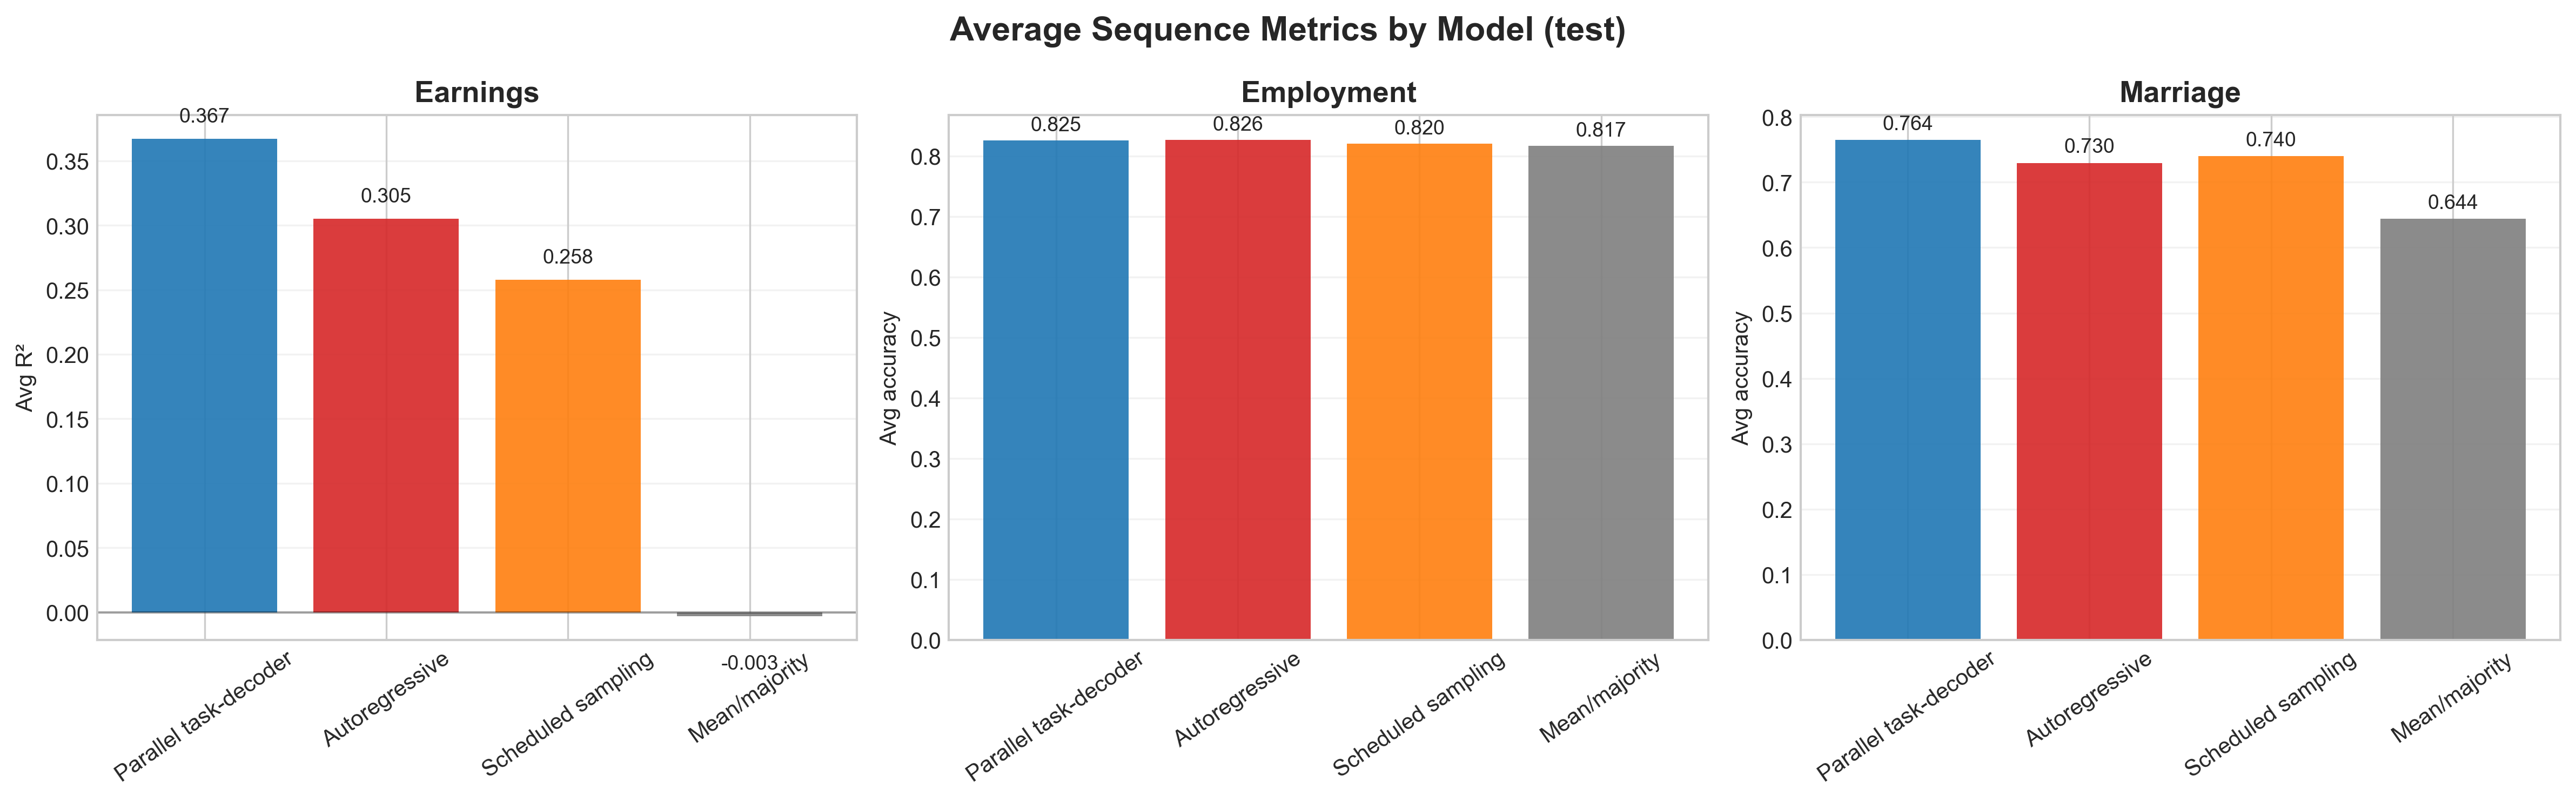
\includegraphics[width=1\linewidth]{../../results/autoregressive_comparison_plots/combined_average_metrics_test.png}
\end{center}
}

\posterblock{Input Ablation}{
\begin{center}
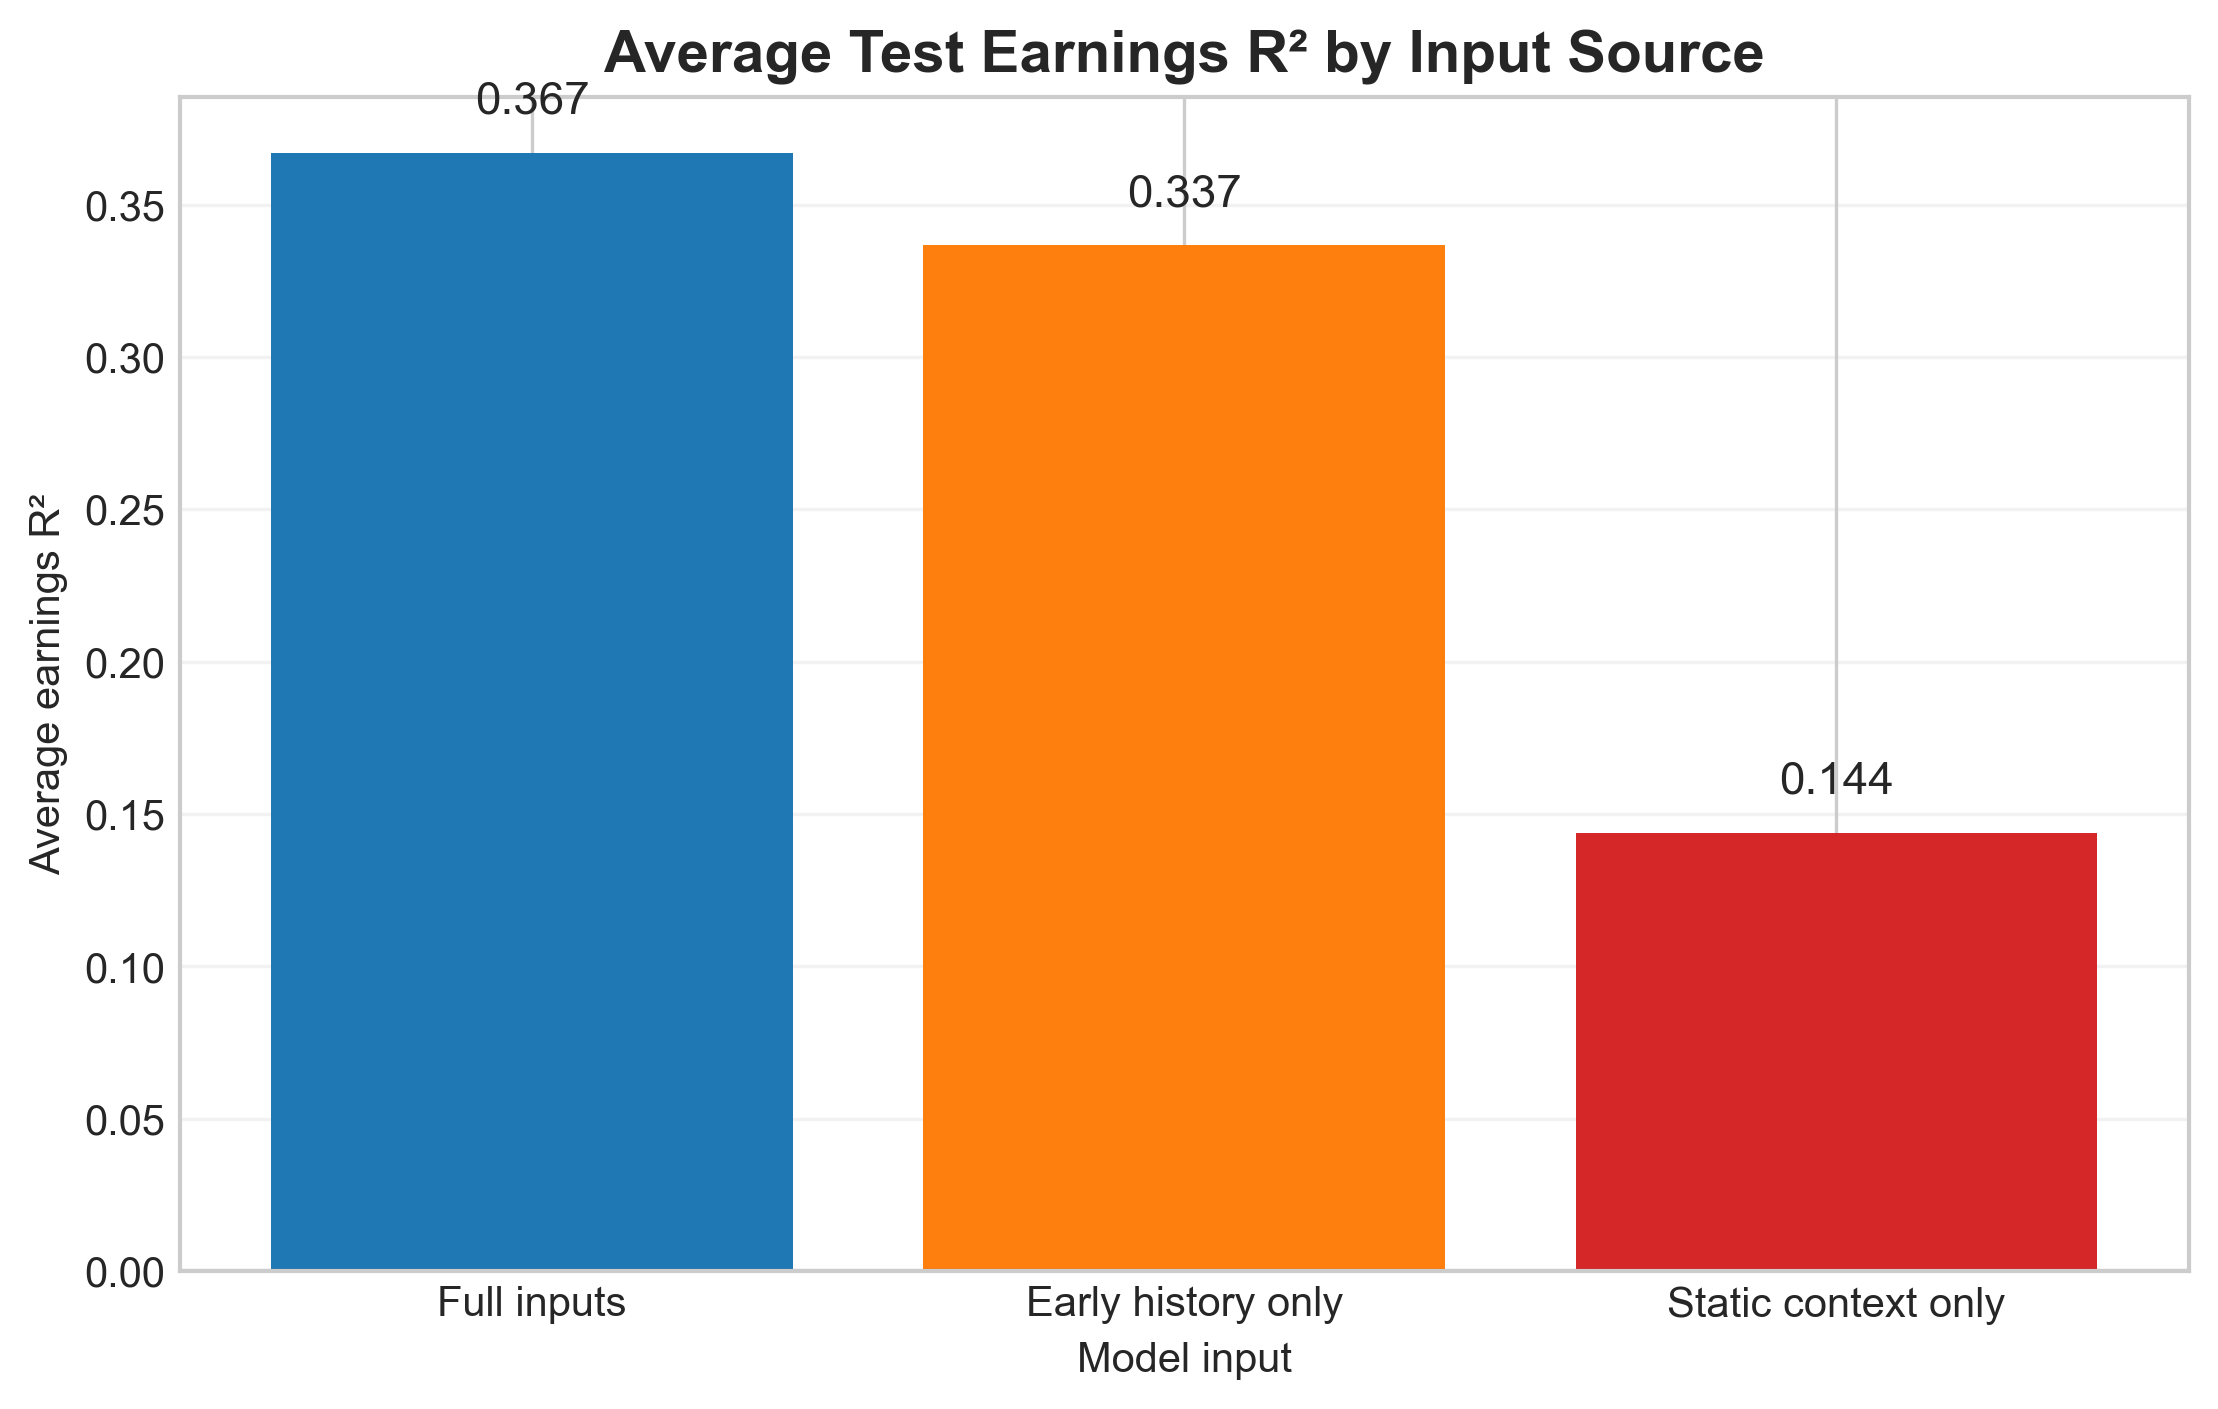
\includegraphics[width=0.75\linewidth]{../../results/task_decoder_ablation_outputs/plots/test_earnings_ablation_average_r2.png}
\end{center}
}

\end{column}

% ----------------------- Column 3 -----------------------
\begin{column}{0.31\textwidth}

\posterblock{Results by Age Bin}{
\begin{center}
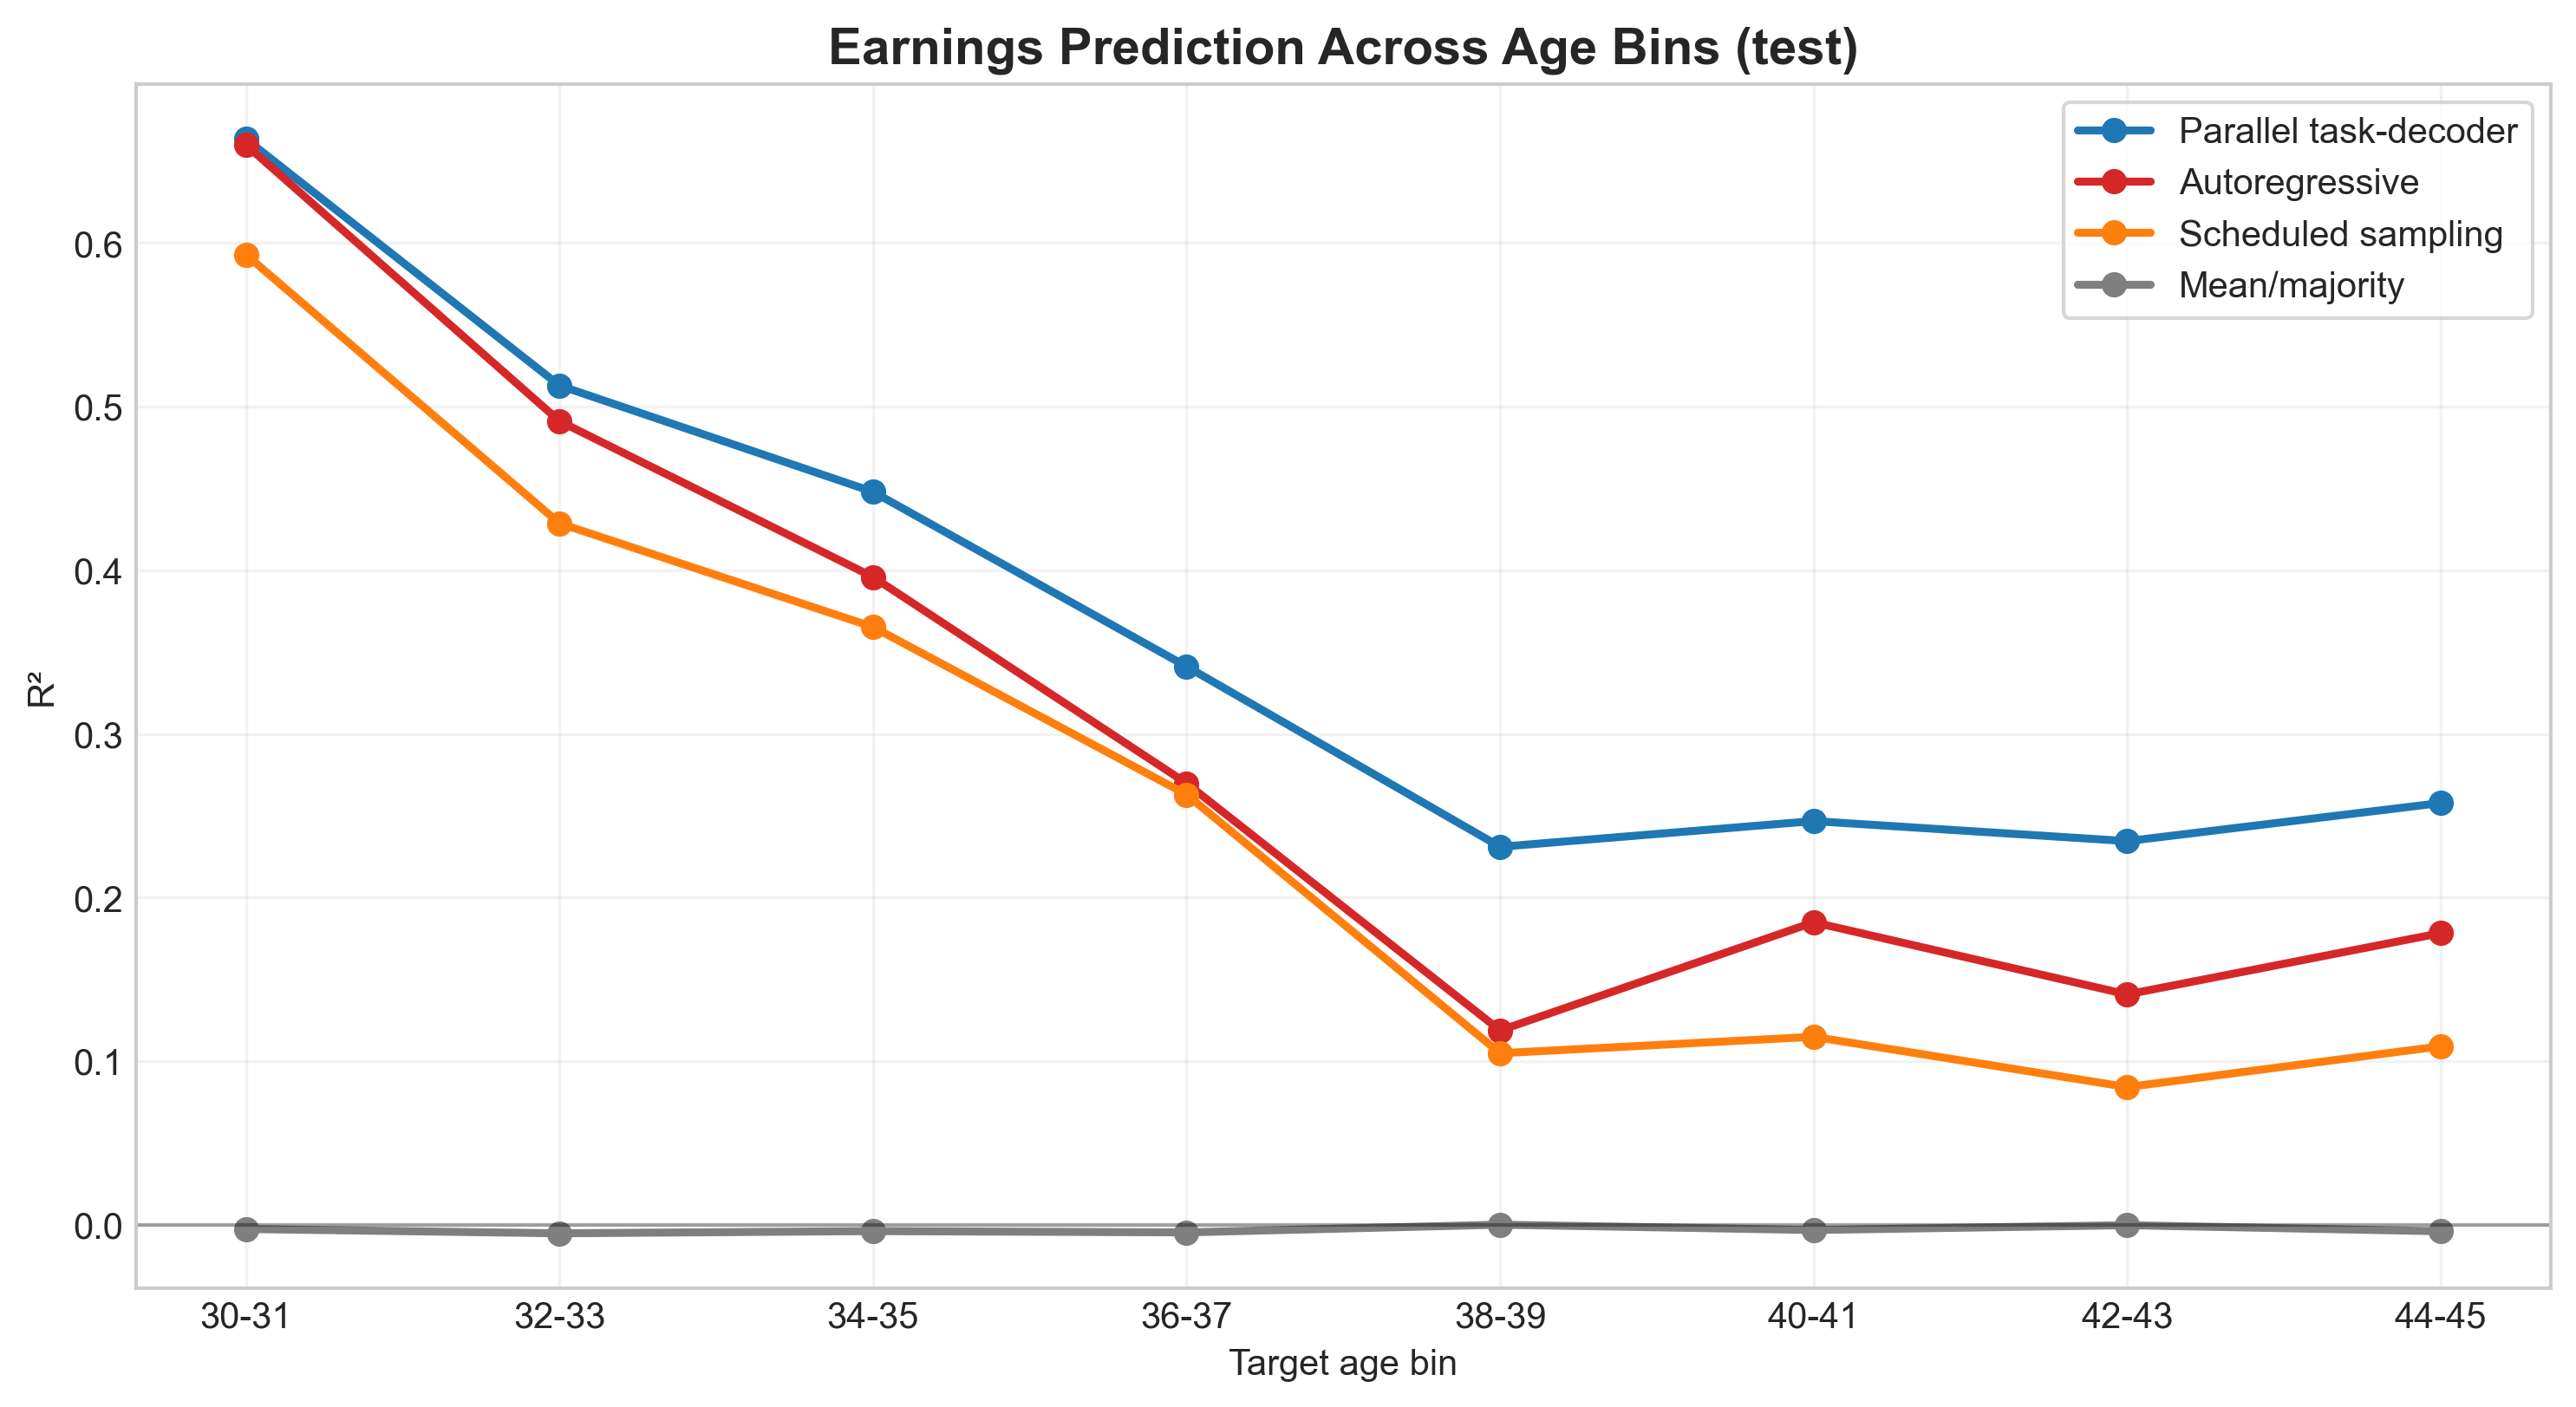
\includegraphics[width=1\linewidth]{../../results/autoregressive_comparison_plots/earn_r2_across_age_test.png}

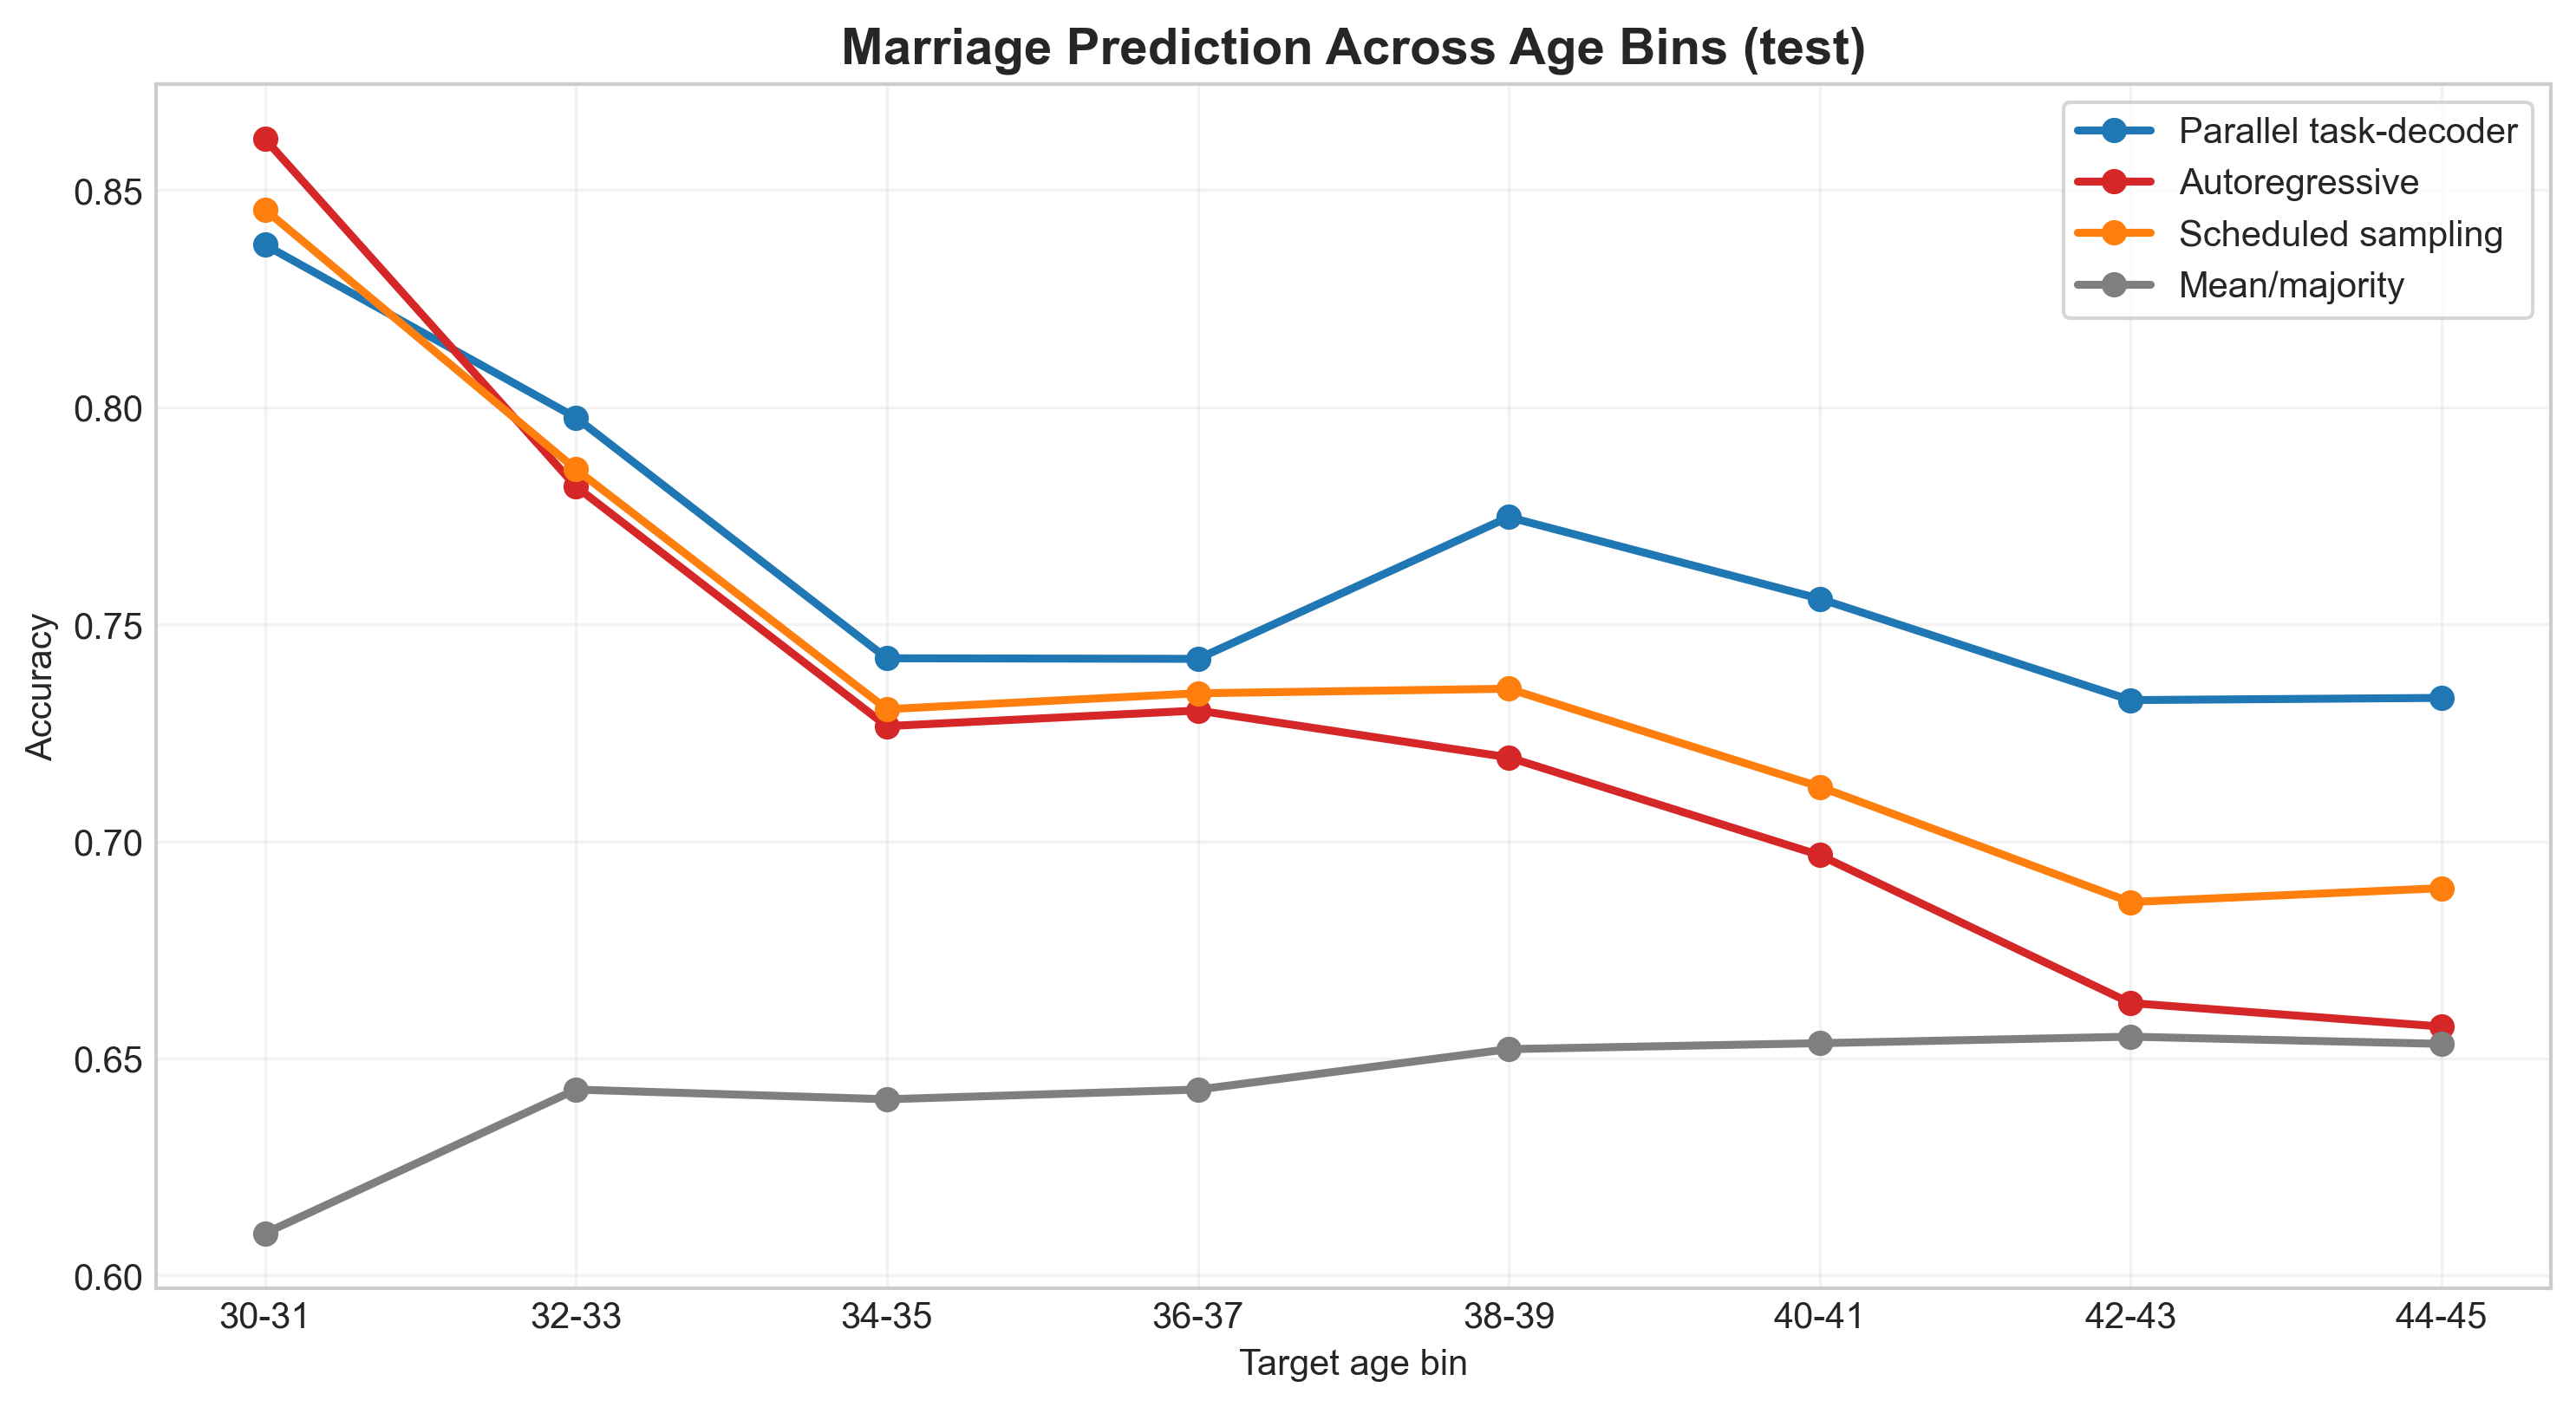
\includegraphics[width=1\linewidth]{../../results/autoregressive_comparison_plots/mar_accuracy_across_age_test.png}
\end{center}
}

\posterblock{Discussion and Future Work}{
\begin{itemize}
  \item Early adult trajectories appear to summarize much of the predictive signal from family background, consistent with a near-Markov interpretation: family background may shape early trajectories, which then mediate later outcomes.
  \item Autoregressive results show a limit of treating life-course prediction like sentence completion. With sparse observations and omitted shocks, generated future states can amplify noise rather than improve long-horizon prediction.
  \item Limitations include small sample size, missingness, irregular timing, and omitted variables such as health, labor markets, and macro-level shocks.
  \item Future work should use larger and richer data with more life-course covariates to improve accuracy.
\end{itemize}
}

\end{column}

\end{columns}

\end{frame}
\end{document}
